\notechapter{N-20260615}{Surface Integrals, Gauss Theorem, and Stokes Theorem}

\section{Why this note is split this way}


\section{Four integrals that look similar but mean different things}

The first task is to separate four objects:
\[
  \iint_S f(x,y,z)\,dS,\qquad
  \iint_S P\,dy\,dz+Q\,dz\,dx+R\,dx\,dy,
\]
\[
  \iiint_\Omega \nabla\cdot F\,dV,\qquad
  \oint_{\partial S}P\,dx+Q\,dy+R\,dz.
\]
The first is a scalar surface integral: it integrates a scalar density over area.  The second is a flux integral: it integrates a vector field through an oriented surface.  The third is the volume integral of divergence.  The fourth is circulation along an oriented boundary curve.

The common mistake is to treat all of them as ``surface integral formulas.''  They are not the same mathematical object.  Their relation is supplied by Gauss' theorem and Stokes' theorem.

\section{First-kind surface integrals}

Let $S$ be a smooth surface parametrized by
\[
  r(u,v)=(x(u,v),y(u,v),z(u,v)),\qquad (u,v)\in D.
\]
Then
\[
  dS=|r_u\times r_v|\,du\,dv,\qquad
  \iint_S f\,dS=\iint_D f(r(u,v))|r_u\times r_v|\,du\,dv.
\]
This is the surface analogue of the first-kind line integral $\int_C f\,ds$.

For a graph $z=z(x,y)$,
\[
  r(x,y)=(x,y,z(x,y)),\qquad
  r_x\times r_y=(-z_x,-z_y,1),
\]
so
\[
  dS=\sqrt{1+z_x^2+z_y^2}\,dx\,dy.
\]
For a graph $x=x(y,z)$ or $y=y(z,x)$, analogous formulas hold:
\[
  dS=\sqrt{1+x_y^2+x_z^2}\,dy\,dz,\qquad
  dS=\sqrt{1+y_z^2+y_x^2}\,dz\,dx.
\]


\begin{figure}[H]
\centering
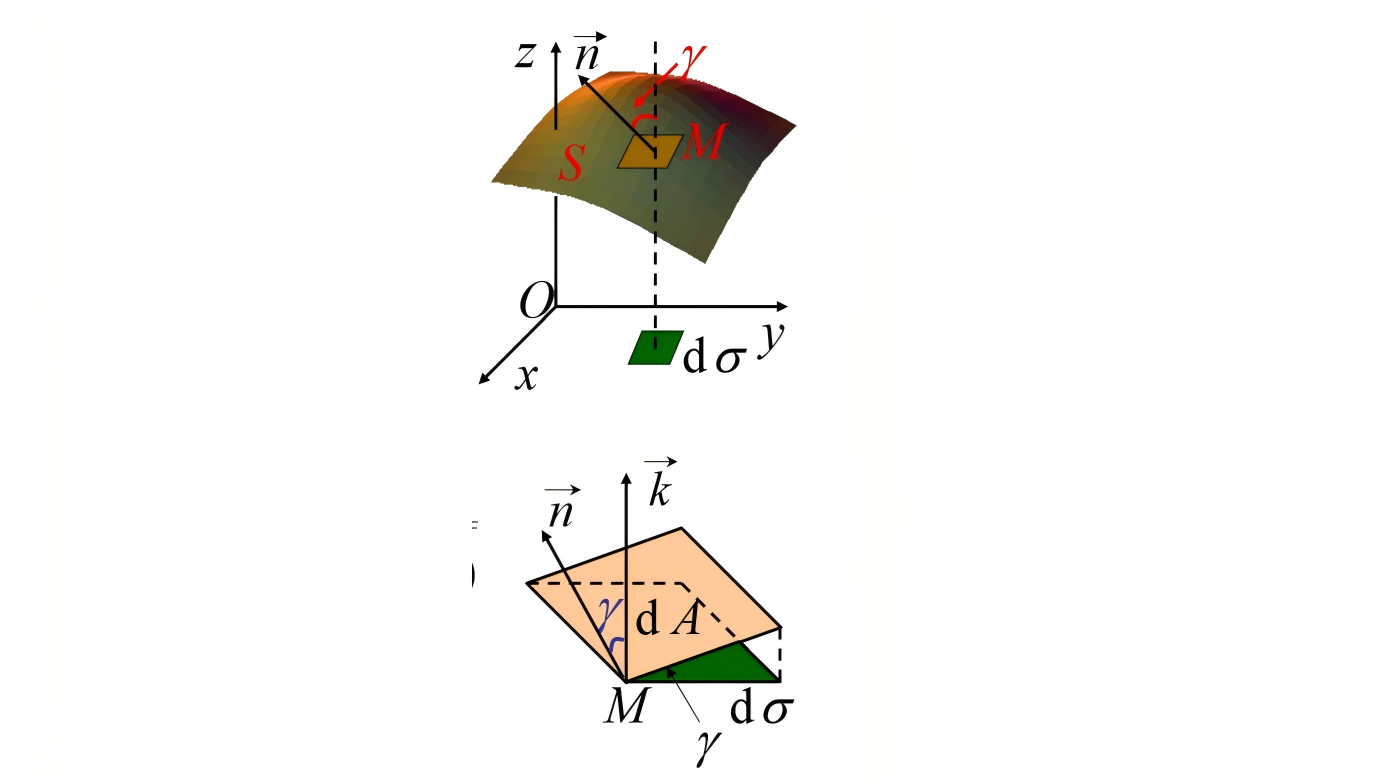
\includegraphics[width=0.86\textwidth,height=0.74\textheight,keepaspectratio]{figures/notes-md/N-20260615/N-20260615-fig-01-surface-area-element-and-projection.png}
\caption{A surface area element and its projection.  The factor between \(dS\) and the projected area element is determined by the angle between the surface normal and the projection direction.}
\end{figure}

\section{Template surfaces}

The original note lists the common templates, and they should be kept because they prevent repeated derivations.

For a plane $z=ax+by+c$,
\[
  dS=\sqrt{1+a^2+b^2}\,dx\,dy.
\]
For a sphere $x^2+y^2+z^2=R^2$, spherical coordinates give
\[
  dS=R^2\sin\varphi\,d\varphi\,d\theta.
\]
For a cylinder $x=R\cos\theta$, $y=R\sin\theta$, $z=z$,
\[
  dS=R\,d\theta\,dz.
\]
For a cone $z=\sqrt{x^2+y^2}$, use $x=r\cos\theta$, $y=r\sin\theta$, $z=r$, so
\[
  |r_r\times r_\theta|=\sqrt2\,r.
\]


\begin{figure}[H]
\centering
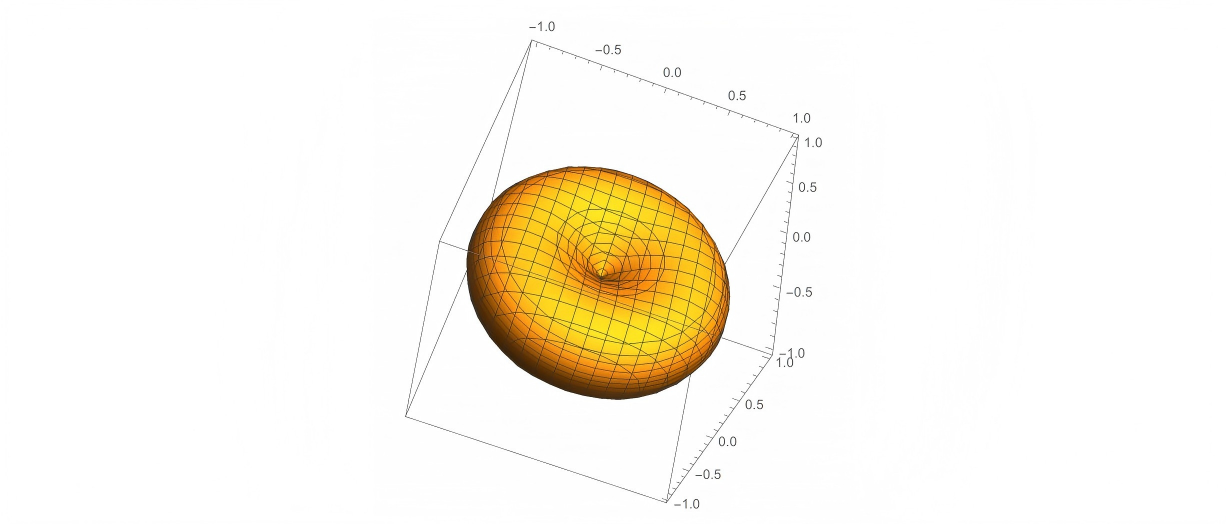
\includegraphics[width=0.70\textwidth,height=0.74\textheight,keepaspectratio]{figures/notes-md/N-20260615/N-20260615-fig-04-torus-example-surface.png}
\caption{A torus as a standard example of a parametrized surface.}
\end{figure}

\section{Example pattern: spherical cap}

For a spherical cap on $x^2+y^2+z^2=R^2$, the scalar integral of $f$ should normally be written in spherical coordinates.  If the cap is cut by $z=h$, then $z=R\cos\varphi$ gives
\[
  0\le\varphi\le \arccos(h/R).
\]
Thus
\[
  \iint_S f\,dS=
  \int_0^{2\pi}\int_0^{\arccos(h/R)}
  f(R\sin\varphi\cos\theta,R\sin\varphi\sin\theta,R\cos\varphi)
  R^2\sin\varphi\,d\varphi\,d\theta.
\]
The important part of the example is not the final antiderivative.  It is recognizing the right parameter domain.

\begin{figure}[H]
\centering
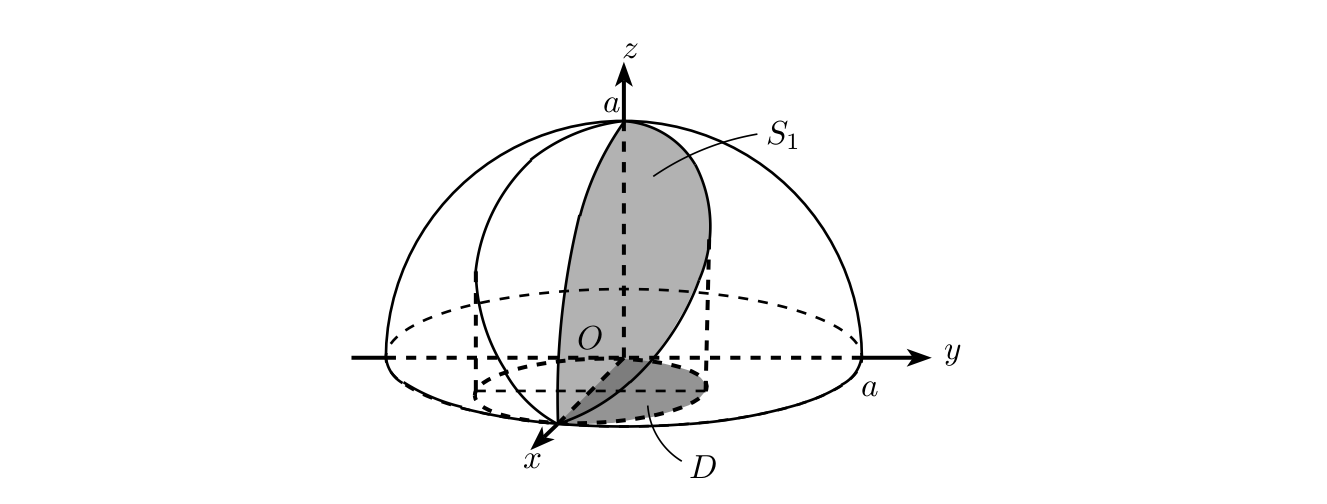
\includegraphics[width=0.78\textwidth,height=0.74\textheight,keepaspectratio]{figures/notes-md/N-20260615/N-20260615-fig-02-spherical-surface-patch-and-projection-domain.png}
\caption{A spherical surface patch and its projection domain.  This is the geometric model behind many spherical-cap surface integrals.}
\end{figure}

\begin{figure}[H]
\centering
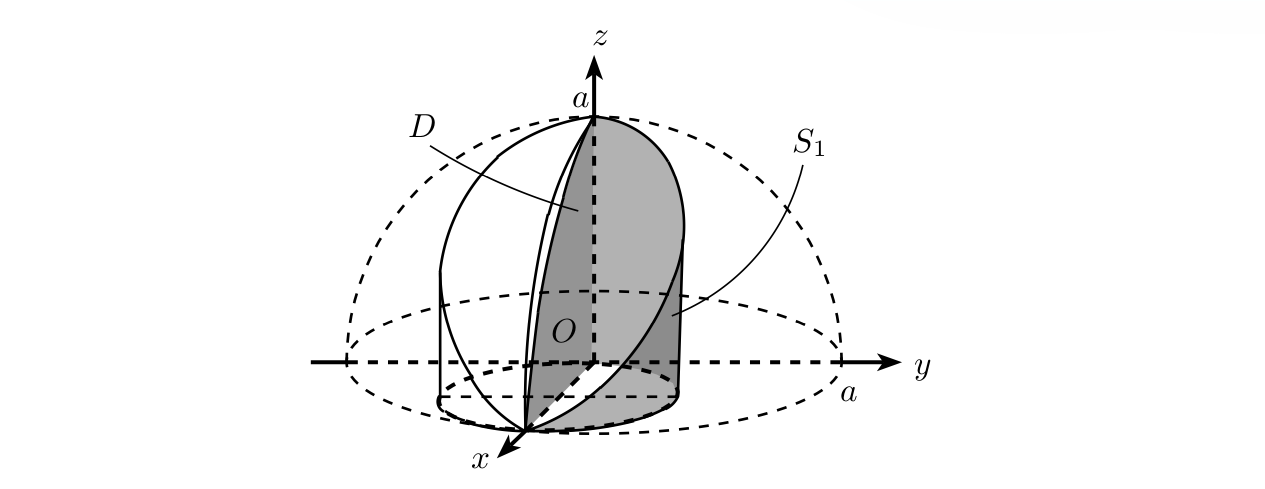
\includegraphics[width=0.78\textwidth,height=0.74\textheight,keepaspectratio]{figures/notes-md/N-20260615/N-20260615-fig-03-spherical-surface-with-bounding-cylinder.png}
\caption{A related spherical surface cut out by a vertical boundary.  The dashed curves indicate the hidden projection and bounding geometry.}
\end{figure}





\section{Second-kind surface integrals as flux}

Let $F=(P,Q,R)$.  The flux through an oriented surface $S$ is
\[
  \iint_S F\cdot n\,dS.
\]
In differential notation this is
\[
  \iint_S P\,dy\,dz+Q\,dz\,dx+R\,dx\,dy.
\]
For a parametrization $r(u,v)$,
\[
  \iint_S F\cdot n\,dS
  =\iint_D F(r(u,v))\cdot(r_u\times r_v)\,du\,dv,
\]
where the order of $u,v$ determines orientation.

For a graph $z=z(x,y)$ with upward orientation,
\[
  n\,dS=(-z_x,-z_y,1)\,dx\,dy,
\]
so
\[
  \iint_S F\cdot n\,dS
  =\iint_D[-Pz_x-Qz_y+R]\,dx\,dy.
\]
For downward orientation, change the sign.

\section{Typical flux examples from the source}

The original long note includes sphere, cone, shifted sphere, rectangular box, and partial-sphere examples.  The common structures are these.

For a sphere with outward orientation, direct parametrization works, but Gauss' theorem is often shorter if the surface is closed.  For a cone with upper orientation, the graph formula or cone parametrization should be used; the sign is the main danger.  For a shifted sphere such as
\[
  (x-a)^2+y^2+z^2=R^2,
\]
translation changes the integrand but not the geometric idea.  For a rectangular box, flux splits over six faces unless Gauss' theorem turns it into one volume integral.  For a sphere piece with only $dx\,dy$, the projection to the $xy$-plane and the sign of the normal decide whether the upper and lower sheets add or cancel.

\section{Gauss theorem}

Let $\Omega$ be a solid with outward boundary $\partial\Omega$.  For $F=(P,Q,R)$,
\[
  \iint_{\partial\Omega}F\cdot n\,dS
  =
  \iiint_\Omega (P_x+Q_y+R_z)\,dV.
\]
The divergence
\[
  \nabla\cdot F=P_x+Q_y+R_z
\]
measures local source strength.  Gauss' theorem says that total source inside equals outward flux through the boundary.

Use Gauss when the surface is closed, or when it can be closed by adding a simple cap.  If the required surface is not closed, compute the closed flux and subtract the flux across the added part.  If the problem asks for inward orientation, multiply the outward result by $-1$.

\section{Singular fields and missing points}

The note includes the important example type where the field is singular at a point.  Gauss' theorem cannot be applied across a singularity.  The usual remedy is to remove a small sphere around the singular point, apply Gauss' theorem to the punctured region, and then let the radius tend to zero.  For inverse-square radial fields, the flux through the small sphere often remains nonzero.  This is the analytic origin of point charges and delta-type sources.

\section{Stokes theorem}

Let $S$ be an oriented surface with boundary $\partial S$.  Then
\[
  \oint_{\partial S}F\cdot dr
  =
  \iint_S (\nabla\times F)\cdot n\,dS.
\]
Here
\[
  \nabla\times F=
  \begin{vmatrix}
  i&j&k\\
  \partial_x&\partial_y&\partial_z\\
  P&Q&R
  \end{vmatrix}.
\]
The right-hand rule fixes orientation: if the thumb points along $n$, the fingers curl in the positive boundary direction.

Use Stokes when the boundary curve is complicated but some spanning surface is simple, or when the curl is much simpler than the original vector field.  The surface can be changed as long as the boundary and orientation are preserved.

\section{Examples preserved from the long note}

For a triangular boundary in a plane, Stokes lets us replace a line integral over three edges by a surface integral over the triangle.  If the curl is constant, the result is just the dot product of the curl with the oriented area vector.

For an elliptical boundary, choose the planar elliptical disk rather than the original curved surface when allowed.  Parameterizing the ellipse directly is usually longer; Stokes rewards choosing the simplest spanning surface.

\section{Decision table}

\begin{center}
\begin{tabular}{lll}
\toprule
Object & Meaning & Best tool \\
\midrule
$\iint_S f\,dS$ & scalar density on surface & parametrization or graph $dS$ \\
$\iint_SF\cdot n\,dS$ & flux through oriented surface & graph formula or Gauss \\
closed flux & total outward flow & Gauss theorem \\
line circulation & work/circulation along boundary & direct line integral or Stokes \\
\bottomrule
\end{tabular}
\end{center}

\section{Conceptual endpoint}

The high-level statement is the boundary principle:
\[
  \int_{\partial M}\omega=\int_M d\omega.
\]
Green, Gauss, and Stokes are all versions of this formula.  The old vector-calculus notation hides the unity; differential forms reveal it.  The derivative $d\omega$ records local change inside a region, and the boundary integral records the accumulated effect at the edge.

\section{Elementary-to-advanced bridge: general Stokes theorem}

The vector-calculus theorems in this note are all cases of the general Stokes theorem.  If $M$ is an oriented smooth manifold with boundary and $\omega$ is a compactly supported differential form of degree one less than $\dim M$, then
\[
  \int_{\partial M}\omega=\int_M d\omega.
\]

Green's theorem, Stokes' theorem, and Gauss' theorem correspond to different degrees and dimensions:
\[
  \begin{array}{lll}
  \text{Green} & M\subseteq\mathbb R^2 & \omega=Pdx+Qdy,\\
  \text{Stokes} & M\text{ a surface in }\mathbb R^3 & \omega=Pdx+Qdy+Rdz,\\
  \text{Gauss} & M\subseteq\mathbb R^3 & \omega=Pdy\wedge dz+Qdz\wedge dx+Rdx\wedge dy.
  \end{array}
\]
The apparently different vector formulas are one theorem written in different degrees.

\section{Elementary-to-advanced bridge: singular sources and distributions}

The note mentions singular fields and missing points.  The advanced language for point sources is distribution theory.  The Dirac delta $\delta_0$ is not an ordinary function but satisfies
\[
  \int \delta_0 \varphi=\varphi(0)
\]
for test functions $\varphi$.

For the inverse-square field in $\mathbb R^3$,
\[
  F(x)=\frac{x}{|x|^3},
\]
one has classically $\nabla\cdot F=0$ away from the origin, but distributionally
\[
  \nabla\cdot F=4\pi \delta_0.
\]
This reconciles the nonzero flux through spheres with zero ordinary divergence away from the singularity.

\section{Elementary-to-advanced bridge: conservation laws}

Many PDEs have conservation-law form
\[
  \partial_t \rho+\nabla\cdot J=0.
\]
Integrating over a region $\Omega$ and applying Gauss' theorem gives
\[
  \frac d{dt}\int_\Omega \rho\,dV=-\iint_{\partial\Omega}J\cdot n\,dS.
\]
Change inside equals negative outward flux.  Thus Gauss' theorem is the geometric mechanism behind conservation of mass, charge, and probability.

\section{Elementary-to-advanced bridge: currents}

A current generalizes an oriented submanifold by acting on differential forms.  An oriented curve $C$ defines a current
\[
  T_C(\omega)=\int_C \omega.
\]
The boundary of a current is defined by
\[
  \partial T(\omega)=T(d\omega).
\]
This extends Stokes' theorem to singular chains, weak surfaces, and geometric measure theory.

The elementary surface and curve integrals in the note are therefore the smooth case of a much more flexible integration theory over generalized geometric objects.

% Second-pass deepening for waves 2-4: wave 4 part 3
\section{Second-pass deepening: Gauss and Stokes as dual local-to-global laws}

Gauss' theorem and Stokes' theorem are both local-to-global principles.  Gauss says that local source density accumulates to boundary flux.  Stokes says that local rotation accumulates to boundary circulation.  In differential-form notation, both are one formula:
\[
  \int_{\partial M}\omega=\int_M d\omega.
\]
The difference lies only in the degree of the form and the dimension of the manifold.

This unification matters because it prevents memorizing vector identities as separate facts.  The object being integrated determines the theorem: a one-form over a boundary curve gives curl through a surface; a two-form over a closed surface gives divergence through a volume.

\section{Second-pass deepening: weak forms and PDE}

In PDE, integration by parts and Stokes-type formulas define weak solutions.  Instead of requiring derivatives to exist pointwise, one tests against smooth functions.  For example, a weak divergence equation is read through
\[
  \int_\Omega F\cdot \nabla \varphi\,dV=-\int_\Omega (\nabla\cdot F)\varphi\,dV
\]
up to boundary terms.

Thus vector-calculus integral theorems are not merely computational shortcuts; they are the foundation of weak formulations, conservation laws, and modern PDE theory.
